\documentclass{xjtubsc}
\usepackage{graphicx}
\usepackage{subfigure} 
% Comments by hy_haoyun
% Note the subfigure is old-fashioned.
% We'd better use subfig instead.
% But I don't have enough time to modify the example.
\usepackage{booktabs}
\usepackage{listings}
\usepackage{xcolor}
\lstset{upquote,
	keepspaces=true,
	columns=spaceflexible,
	basicstyle=\ttfamily\footnotesize,%
	breaklines=true,
	breakindent=0pt,
	xleftmargin=0pt,
	xrightmargin=6pt,%
	language=matlab,
	commentstyle=\sffamily\itshape\color{SeaGreen4},
	emphstyle=\bfseries\color{RoyalBlue3},escapechar={`'},
	emphstyle={[2]{\bfseries\color{Sienna2}}},
}
\graphicspath{{figures/}}
\begin{document}

 \noindent {\bf \zihao{-4}
论文题目:毕设模板说明书\\
学生姓名:王鸿鑫、秦雨果\\
指导教师:郝运\\ }
\begin{chabstract}
这是毕设模板的说明书,如果有问题,请到这里来找答案,我们希望帮助你漂亮的呈现自己的成果。
\end{chabstract}
\chkeywords{中文;模板;说明书}
 \noindent {\bf \zihao{-4}
Title:Template manual\\
Name:wanghongxin,qinyuguo\\
Supervisor:haoyun\\ }
\begin{enabstract}
This is the manual of the template.
\end{enabstract}
\enkeywords{English;template;manual}

\tableofcontents

% Comment by hy_haoyun:
%	1. 目录的页码应该是罗马的。

\newpage
\mainbodyformat
\section{绪论}
正文是学位论文的主体,第一章为绪论,最后一章为结论与展望。我们来测试一个上标引用。为什么要写这篇论文,要解决什么问题,主要观点是什么。 对本论文研究主题范围内已有文献的评述(包括与课题相关的历史的回顾,资料来源、性质及运用情况等)。说明本论文所要解决的问题,所采用的研究手段、方式、方法。明确研究工作的界限和规模。概括论文的主要工作内容。

我们其实已经不知不觉地到达了终点。不幸的是,我们经过20 多
年辛苦跋涉所到达的这个终点,并不是什么美丽的“新世界”,而是中国历史上反复出现过的旧朝代的翻版。王亚南先生早在半个世纪之前就在它那部研究中国官僚体系的开山之作中提醒我们,中国源远流长的官僚政治体系有着神奇的亲和力,它可以与任何体制相互融合。它既可以与古老的小农经济,也可以与现代意义上的自由市场或者国家资本主义相结合;它既能够将儒释道汇于一炉,也能够将现代三民主义、法西斯主义杂糅并蓄之后,自成一体。而当今世界的这个主义,那个主义自然同样不在话下。这或许正是中国官僚政治自秦以降,能够绵绵延续
2000年的关键原因。正所谓“2000年之政,秦政也,皆大盗也。
\begin{figure}[H]
\centering
\subfigure[原始图像]{\label{figure:001} 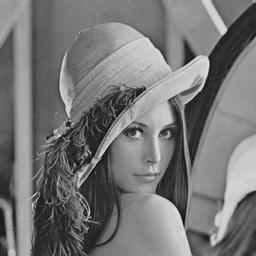
\includegraphics[width=0.2\textwidth]{001}}
\subfigure[噪声图像($\mu=0,\sigma=20$)]{\label{figure:002} 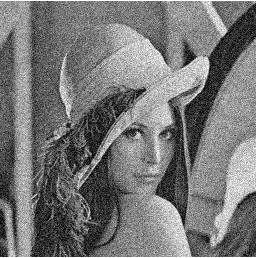
\includegraphics[width=0.2\textwidth]{002}}
\caption{初始图像}
\end{figure}

\begin{figure}[H]
\centering
\subfigure[$\lambda=\frac{1}{20^2}$]{\label{figure:1/20}
 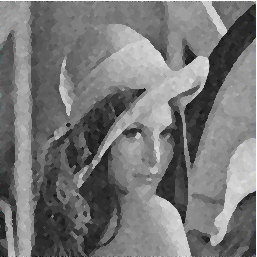
\includegraphics[width=0.2\textwidth]{003}}
\subfigure[$\lambda=\frac{5}{20^2}$]{\label{figure:5/20} 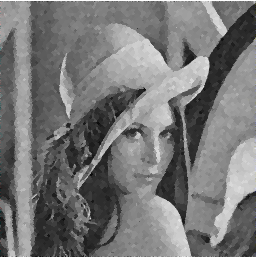
\includegraphics[width=0.2\textwidth]{004}}
\subfigure[$\lambda=\frac{10}{20^2}$]{\label{figure:10/20} 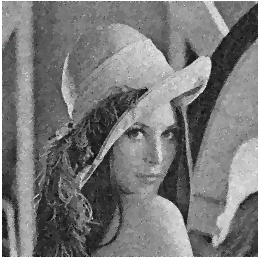
\includegraphics[width=0.2\textwidth]{005}}
\subfigure[$\lambda=\frac{20}{20^2}$]{\label{figure:20/20} 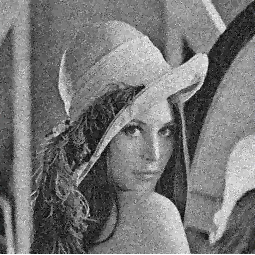
\includegraphics[width=0.2\textwidth]{006}}
\caption{处理的像}
\end{figure}   

    每章标题按一级标题编排,每节标题按二级标题编排,每小节标题按三级标题编排。
    
\subsection{参考文献}
\label{sec:bib}
当然参考文献可以直接写~bibitem,虽然费点功夫,但是好控制,各种格式可以自己随意改
写。

本模板推荐使用~BIB\TeX,样式文件为~thubib.bst,基本符合学校的参考文献格式(如专利
等引用未加详细测试)。看看这个例子,关于书的
\cite{tex, companion, ColdSources},
还有这些 \cite{Krasnogor2004e, clzs, zjsw},关于杂志的\cite{ELIDRISSI94,
  MELLINGER96, SHELL02},硕士论文 \cite{zhubajie, metamori2004},博士论文 \cite{shaheshang, FistSystem01},标准文件\cite{IEEE-1363},会议论文 \cite{DPMG,kocher99},技术报告\cite{NPB2}。中文参考文献\cite{cnarticle}应增~\texttt{lang=``zh''}~字段,以便进行相应处理。另外,这个~bst 对中文文献\cite{cnproceed}的支持并不是十全十美,如果有不如意的地方,请手动修改~bbl 文件。

    \begin{table}[htb]
  \centering
  \begin{minipage}[t]{0.8\linewidth} 
  % 如果想在表格中使用脚注,minipage是个不错的办法
  \caption[模板文件]{模板文件。如果表格的标题很长,那么在表格索引中就会很不美
    观,所以要像~chapter 那样在前面用中括号写一个简短的标题。这个标题会出现在索
    引中。}
  \label{tab:template-files}
    \begin{tabular*}{\linewidth}{lp{10cm}}
      \toprule[1.5pt]
      {\bf文件名} & {\bf 描述} \\\midrule[1pt]
      thuthesis.ins & \LaTeX{} 安装文件,docstrip\footnote{表格中的脚注} \\
      thuthesis.dtx & 所有的一切都在这里面\footnote{再来一个}。\\
      thuthesis.cls & 模板类文件。\\
      thuthesis.cfg & 模板配置文。cls 和~cfg 由前两个文件生成。\\
      thubib.bst    & 参考文献~Bibtex 样式文件。\\
      thutils.sty   & 常用的包和命令写在这里,减轻主文件的负担。\\
      \bottomrule[1.5pt]
    \end{tabular*}
  \end{minipage}
\end{table}

    “章”、“节”、“小节”的编号统一为:1、1.1、1.1.1。
    
\begin{equation}
\frac{x}{y}
\end{equation}


    四级以后的标题和编号的编排原则为:下级标题的显目程度不超过上一级,不重复或混淆。

    编号与题目之间空一格。

    \subsection{二级标题}
    

        积土成山,风雨兴焉;积水成渊,蛟龙生焉;积善成德,而神明自得,圣心备焉。故不积跬步,无以至千里;不积小流,无以成江海。骐骥一跃,不能十步;驽马十驾,功在不舍。锲而舍之,朽木不折;锲而不舍,金石可镂。蚓无爪牙之利,筋骨之强,上食埃土,下饮黄泉,用心一也。蟹六跪而二螯,非蛇鳝之穴无可寄托者,用心躁也。
         

        \subsection{三级标题}

        平林漠漠烟如织,寒山一带伤心碧。暝色入高楼,有人楼上愁。王阶空伫立,宿鸟归飞急。何处是归程,长亭更短亭。


            \subsubsection{四级标题}
                
            君不见,黄河之水天上来,奔流到海不复回。君不见,高堂明镜悲白发,朝如青丝暮成雪。人生得意须尽欢,莫使金樽空对月。天生我材必有用,千金散尽还复来。烹羊宰牛且为乐,会须一饮三百杯。岑夫子,丹丘生,将进酒,君莫停。与君歌一曲,请君为我侧耳听。钟鼓馔玉不足贵,但愿长醉不复醒。古来圣贤皆寂寞,惟有饮者留其名。陈王昔时宴平乐,斗酒十千恣欢谑。主人何为言少钱,径须沽取对君酌。五花马,千金裘,呼儿将出换美酒,与尔同销万古愁。

            \subsubsection{四级标题}

                一屠晚归,担中肉尽,止有剩骨。途中两狼,缀行甚远。

                屠惧,投以骨。一狼得骨止,一狼仍从。复投之,后狼止而前狼又至。骨已尽矣,而两狼之并驱如故。

                屠大窘,恐前后受其敌。顾野有麦场,场主积薪其中,苫蔽成丘。屠乃奔倚其下,弛担持刀。狼不敢前,眈眈相向。

                少时,一狼径去,其一犬坐于前。久之,目似瞑,意暇甚。屠暴起,以刀劈狼首,又数刀毙之。方欲行,转视积薪后,一狼洞其中,意将隧入以攻其后也。身已半入,止露尻尾。屠自后断其股,亦毙之。乃悟前狼假寐,盖以诱敌。

                狼亦黠矣,而顷刻两毙,禽兽之变诈几何哉?止增笑耳。

            \subsubsection{又是一个四级标题}

                孔子东游,见两小儿辩斗。问其故。

                一儿曰:“我以日始出时去人近,而日中时远也。”

                一儿以日初出远,而日中时近也。

                一儿曰:“日初出大如车盖,及日中则如盘盂,此不为远者小而近者大乎?”

                一儿曰:“日初出沧沧凉凉,及其日中如探汤,此不为近者热而远者凉乎?”

                孔子不能决也。

                两小儿笑曰:“孰为汝多知乎?”


\section{理论分析}
\subsection{问题重述}
我们首先引入线性算子
\begin{align*}
&R:L^2(\Omega) \longrightarrow L^2(\Omega) \\
Ru(x,y)=&\int_\Omega K(x-x^1,y-y^1)u(x^1,y^1)dx^1dy^1
\end{align*}
其中 $K(x,\epsilon,y,\tau)$ 为脉冲响应函数,并且我们总假定线性算子 $R$ 是有界的。

若已知 $u$ 的模糊版本 $g$,则由方程 $g=Ru$ 求 $u$ 是一个典型的反问题,称为图像去模糊问题或图像去卷积\footnote{算子}。这里我们考虑含加性噪声的图像 $u_0$,含加性噪声的模糊图像 $u_0$ 满足方程
\[u_0=Ru+\eta\]
其中: $\eta$ 表示高斯白噪声,即
\[\int_\Omega \eta(x)=0,\int_\Omega \eta^2(x)=\sigma^2\]
综上所述,这里考虑的基本问题是:已知初值数据 $u_0$,算子 $R:L^2(\Omega) \longrightarrow L^2(\Omega)$ 是有界线性算子,图像噪声方差 $\sigma^2$,根据含噪声模糊图像模型
\[u_0=Ru+\eta\]
重建或者复原 $u$,特别的,当 $R$ 为恒同算子时,基本问题\footnote{什么}就称为去噪问题。

\subsection{问题分析}
以下我们考虑当 $R$ 为恒同算子时的去噪问题,即
\begin{equation}
u_0=u+\eta
\end{equation}
其中: $\eta$ 表示高斯白噪声,即
\begin{equation}
\label{zaosheng}
E\eta(x)=0,E\eta^2(x)=\sigma^2
\end{equation}
由噪声式 (\ref{zaosheng}) 的假设导致了两种约束
\begin{align}
\iint\limits_\Omega u(x,y)\,dx\,dy =\iint\limits_\Omega u_0(x,y)\,dx\,dy\\
\frac{1}{|\Omega|}\iint\limits_\Omega (u(x,y)-u_0(x,y))^2\,dx\,dy =\sigma^2
\end{align}
其中 $|\Omega|$ 为图像区域 $\Omega$ 的面积。

由Rudin、Osher 和Fatemi提出的 TV 图像复原模型,是图像复原中最成功的方法。与最小二乘复原模型相比,TV 模型最主要的差别是用梯度的 Ll 范数替代了它的 L2 范数,也就是最小化全变分(Rudin 认为,有噪声图像的全变分比无噪声图像的全变分明显大,最小化全变分可以消除噪声)。

令 $F_1(u)=\int_\Omega 2|\triangledown u|^{\frac{1}{2}}dxdy$,由于 $F_1(u)$ 具有平移不变性,即 $F_1(u+c)=F_1(u)$,$c$ 为任意常数,那么第一个约束实际上是自满足的。因此,通常我们只需要考虑第二个拟合约束。通过引入拉格朗日乘子 $\lambda$,可以定义一个新的能量泛函:
\begin{equation}
\label{nengliangfanhan}
J(u)=\int_\Omega 2|\triangledown u(x,y)|^{\frac{1}{2}} dxdy +\frac{\lambda}{2} \int_\Omega |u-u_0|^2dxdy
\end{equation}
其中,参数 $\lambda$ 对平衡去噪与平滑起重要作用。这是一个泛函求极值问题,即变分问题。

\subsection{PDE的推导}
从 (\ref{nengliangfanhan}) 式中可以看出该能量泛函为
\begin{equation}
J(u)=\int_\Omega F(x,y,u,\frac{\partial u}{\partial x},\frac{\partial u}{\partial y}) dxdy
\end{equation}
型泛函,其中
\begin{equation}
\label{Ffanhan}
F= 2|\triangledown u(x,y)|^{\frac{1}{2}}+\frac{\lambda}{2}|u-u_0|^2
\end{equation}
由泛函求极值的必要条件,有欧拉—拉格朗日方程(PDE)
\begin{equation}
\label{EL}
F_H-\frac{\partial}{\partial x}\{F_p\}-\frac{\partial}{\partial y}\{F_q\} =0
\end{equation}
其中 $p=\frac{\partial u}{\partial x},q=\frac{\partial u}{\partial y}$。所以对于 (\ref{Ffanhan})式有
\begin{equation}
F_H=\lambda(u-u_0),F_p=\frac{\frac{\partial u}{\partial x}}{|\triangledown u|^{\frac{3}{2}}},F_q=\frac{\frac{\partial u}{\partial y}}{|\triangledown u|^{\frac{3}{2}}}
\end{equation}
将上式代入式(\ref{EL}) 有:
\begin{align*}
\lambda (u-u_0)-\Big\{\frac{\partial}{\partial x}\Big\{\frac{\frac{\partial u}{\partial x}}{|\triangledown u|^{\frac{3}{2}}}\Big\}+\frac{\partial}{\partial y}\Big\{\frac{\frac{\partial u}{\partial x}}{|\triangledown u|^{\frac{3}{2}}}\Big\}\Big\}&=0 \\
\lambda (u-u_0)-\Big(\frac{\partial}{\partial x},\frac{\partial}{\partial y}\Big)\cdot \Big(\frac{\frac{\partial}{\partial x}}{|\triangledown u|^\frac{3}{2}},\frac{\frac{\partial}{\partial y}}{|\triangledown u|^\frac{3}{2}}\Big)&=0
\end{align*}
综上得到该模型的欧拉—拉格朗日方程(PDE):
\begin{equation}
\label{EL1}
-\triangledown \cdot (|\triangledown u|^{-\frac{3}{2}} \triangledown u)+\lambda (u-u_0)=0
\end{equation}
同理,对于能量泛函
\begin{equation}
J(u)=\int_\Omega \frac{1}{p}|\triangledown u(x,y)|^p dxdy +\frac{\lambda}{2} \int_\Omega |u-u_0|^2dxdy,0<p<2
\end{equation}
我们有对应的欧拉—拉格朗日方程(PDE):
\begin{equation}
-\triangledown \cdot (|\triangledown u|^{p-2} \triangledown u)+\lambda (u-u_0)=0
\end{equation}

\subsection{模型的数值实现}
通过前面的分析知道,求解变分问题式 (\ref{nengliangfanhan}) 与求解偏微分方程 (\ref{EL1})是等价的。我们在这里通过差分迭代法直接求解相关的平衡方程(稳定解)。

首先对图像进行等间隔采样,设采样步长 $h=1$。设目标像素为 $u(i,j),A=\big\{ (i,j+1),(i-1,j),(i,j-1),(i+1,j)\big\}$ 为目标像素 $u(i,j)$ 的四个邻域点位置的集合,如下图所示。$e,n,w,s$ 为对应的四个半像素点,它们不能直接从数字图像中得到。由于 $|\triangledown u|^{\frac{3}{2}}$ 出现在分母,为了避免它为零,我们引入一个小的正参数 $\epsilon$,使得$|\triangledown u|_\epsilon=\sqrt{\epsilon^2+|\triangledown u|^2}$。 只要保持 $\epsilon$ 足够小,便不会影响复原的性能。
\setlength{\unitlength}{0.8cm}
\begin{picture}(6,7.5)
\thicklines
\put(4,4.5){\circle*{0.2}}
\put(4,2.5){\circle*{0.2}}
\put(2,4.5){\circle*{0.2}}
\put(4,6.5){\circle*{0.2}}
\put(6,4.5){\circle*{0.2}}
\put(3,4.5){\circle*{0.2}}
\put(4,3.5){\circle*{0.2}}
\put(4,5.5){\circle*{0.2}}
\put(5,4.5){\circle*{0.2}}
\put(2,4.5){\line(1,0){4}}
\put(4,2.5){\line(0,1){4}}
\put(1,4.7){$(i-1,j)$}
\put(4,2){$(i,j-1)$}
\put(4.2,4.7){$(i,j)$}
\put(6.2,4.5){$(i+1,j)$}
\put(4,6.7){$(i,j+1)$}
\put(3,4.2){$w$}
\put(4.2,3.5){$s$}
\put(4.2,5.5){$n$}
\put(5,4.2){$e$}
\put(0.5,1){图1:目标像素 $(i,j)$ 与它的邻域}
\end{picture}

为了对式(\ref{EL1})进行数值实现,我们先令
\[v=(v^1,v^2)=\frac{\triangledown u}{|\triangledown u|_{\epsilon}^{\frac{3}{2}}}\]
那么旋度 $\triangledown \cdot$ 由差分表示为
\begin{equation}
\triangledown \cdot v=\frac{\partial v^1}{\partial x}+\frac{\partial v^2}{\partial y} \approx (v_e^1-v_w^1)+(v_n^2-v_s^2)
\end{equation}
下面给出 $v_e^1,v_w^1,v_n^2,v_s^2$ 的四个逼近:
\begin{align*}
v_e^1&=\frac{1}{|\triangledown u_e|_\epsilon^{\frac{3}{2}}}\Big[\frac{\partial u}{\partial x}\Big]_e \approx \frac{1}{|\triangledown u_e|_\epsilon^{\frac{3}{2}}} [u(i+1,j)-u(i,j)] \\
|\triangledown u_e|_\epsilon^{\frac{3}{2}}& \approx (\epsilon^2+[u(i+1,j)-u(i,j)]^2+[\frac{u(i+1,j+1)-u(i+1,j-1)}{2}]^2)^{\frac{3}{4}}
\end{align*}
同理可得:
\begin{align*}
v_w^1&=\frac{1}{|\triangledown u_w|_\epsilon^{\frac{3}{2}}}\Big[\frac{\partial u}{\partial x}\Big]_w \approx \frac{1}{|\triangledown u_w|_\epsilon^{\frac{3}{2}}} [u(i,j)-u(i-1,j)] \\
v_n^2&=\frac{1}{|\triangledown u_n|_\epsilon^{\frac{3}{2}}}\Big[\frac{\partial u}{\partial y}\Big]_n \approx \frac{1}{|\triangledown u_n|_\epsilon^{\frac{3}{2}}} [u(i,j+1)-u(i,j)] \\
v_s^2&=\frac{1}{|\triangledown u_s|_\epsilon^{\frac{3}{2}}}\Big[\frac{\partial u}{\partial y}\Big]_s \approx \frac{1}{|\triangledown u_s|_\epsilon^{\frac{3}{2}}} [u(i,j)-u(i,j-1)]
\end{align*}
所以有
\begin{equation}
-\triangledown \cdot (|\triangledown|^{-\frac{3}{2}} \triangledown u)=-\triangledown v=\sum_{q \in A}|\triangledown u_q|_\epsilon^{-\frac{3}{2}}[u(i,j)-u(q)]
\end{equation}
其中,我们定义
\begin{align}
\text{若}  q=(i-1,j),\text{则} p=(i-\frac{1}{2},j) \\
\text{若}  q=(i+1,j),\text{则} p=(i+\frac{1}{2},j) \\
\text{若}  q=(i,j-1),\text{则} p=(i,j-\frac{1}{2}) \\
\text{若}  q=(i,j+1),\text{则}  p=(i,j+\frac{1}{2})
\end{align}

因此式 (\ref{EL1})可转化为
\begin{equation}
\sum_{q \in A} |\triangledown u_p|_\epsilon^{-\frac{3}{2}}[u(i,j)-u(q)]+\lambda (i,j)[u(i,j)-u_0(i,j)]=0
\end{equation}
则可推出:
\begin{equation}
\label{ushi}
u(i,j)=\frac{\sum_{q \in A} |\triangledown u_p|_\epsilon^{-\frac{3}{2}}}{\lambda (i,j)+\sum_{q \in A} |\triangledown u_p|_\epsilon^{-\frac{3}{2}}}u(q)+\frac{\lambda (i,j)}{\lambda (i,j)+\sum_{q \in A} |\triangledown u_p|_\epsilon^{-\frac{3}{2}}}u_0(i,j)
\end{equation}
令
\begin{align}
\label{omega}
\omega_q&=\frac{1}{|\triangledown u_p|_\epsilon^{\frac{3}{2}}} \\
\label{hq}
h_q&=\frac{\omega_q}{\lambda (i,j)+\sum_{q \in A} \omega _q} \\
\label{h0}
h_0&=\frac{\lambda (i,j)}{\lambda (i,j)+\sum_{q \in A} \omega _q}
\end{align}
那么式(\ref{ushi})变为
\begin{equation}
u(i,j)=\sum_{q \in A}h_qu(q)+h_0u_0(i,j)
\end{equation}
其中
\begin{equation}
h_0+\sum_{q \in A}h_q=1
\end{equation}
采用 Gauss-Seidel 迭代法,在每一步 $n$:
\begin{equation}
\label{diedai}
u(i,j)^{(n)}=\sum_{q \in A}h_q^{(n-1)}u(q)^{(n-1)}+h_0^{(n-1)}u_0(i,j)
\end{equation}
综上有图像去噪的算法如下:
\begin{figure}[H]
\centering
\subfigure[$\lambda=\frac{1}{20^2}$]{\label{figure:1/20} 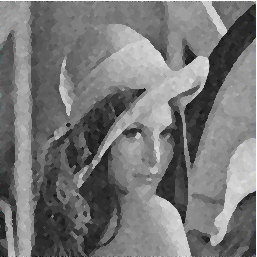
\includegraphics[width=0.4\textwidth]{003}}
\subfigure[$\lambda=\frac{5}{20^2}$]{\label{figure:5/20} 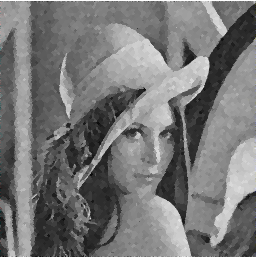
\includegraphics[width=0.4\textwidth]{004}}
\caption{第二章,第一组实验图}
\end{figure}
\begin{tabular}{|p{10cm}|}
\hline
初始化 $u^{(0)}$,通常取 $u^{(0)}=u_0$ ;\\
for $n=1,2,\cdots$  \\
 \quad for $i=1,2,\cdots,M$  \\
   \qquad for $j=1,2,\cdots,N$   \\
根据式 (\ref{omega}),(\ref{hq}),(\ref{h0})分别计算以 $(i,j)$ 为中心点的 $\omega_q,h_q,h_0$,然后利用
式 (\ref{diedai})计算 $u^{(n)}(i,j)$;\\
End \\
\quad End \\
    \qquad End \\
\hline
\end{tabular}
\section{其他工具}
\label{ch3}

\subsection{摘要}
\label{ch3_1}
\subsubsection{中文摘要}
中文摘要在''pages/chabstract.tex''文件中,内容如下
\begin{lstlisting}[frame=single,escapeinside='']
 \noindent {\bf \zihao{-4}
'论文题目:毕设模板说明书'\\
'学生姓名:王鸿鑫、秦雨果'\\
'指导教师:郝运'\\ }
\begin{chabstract}
'这是毕设模板的说明书,如果有问题,请到这里来找答案,我们希望帮助你漂亮的呈现自己的成果。'
\end{chabstract}
\chkeywords{'中文;模板;说明书'}
\end{lstlisting}
效果就如本说明书的摘要。\par

\subsubsection{英文摘要}
英文摘要在''pages/enabstract.tex''文件中,内容如下
\begin{lstlisting}[frame=single,escapeinside='']
 \noindent {\bf \zihao{-4}
Title:Template manual\\
Name:wanghongxin,qinyuguo\\
Supervisor:haoyun\\ }
\begin{enabstract}
This is the manual of the template.
\end{enabstract}
\enkeywords{English;template;manual}
\end{lstlisting}
效果如本说明书的英文摘要。\par

\subsection{附录}
\label{ch3_2}
附录文件开头部分是下面这个样子的
\begin{lstlisting}[frame=single,escapeinside='']
\appendixs{testref.bib'文件'}
\label{appen1}
\begin{lstlisting}[frame=single,escapeinside='']
@book{IEEE-1363,
  author={IEEE Std 1363-2000 and BBB and CCC and DDD},
  title={IEEE Standard Specifications for Public-Key Cryptography},
  type = {M},
  edition = "2",
\end{lstlisting}
效果如附录\ref{appen1},强调一下,附录由
\begin{lstlisting}[frame=single,escapeinside='']
\appendixs{title}
\end{lstlisting}
开始。\par

\subsection{主要符号表}
\label{ch3_3}
主要符号表由如下环境生成
\begin{lstlisting}[frame=single,escapeinside='']
\begin{denotation}
\item[label1]
\item[label2]
\end{denotation}
\end{lstlisting}
比如生成本说明主要符号表的文件``pages/denotation.tex''内容如下
\begin{lstlisting}[frame=single,escapeinside='']
\begin{denotation}
\item[HPC] '高性能计算~(High Performance Computing)'
\item[cluster] 集群
\item[Itanium] 安腾
\item[SMP] 对称多处理
\item[API] 应用程序编程接口
\item[PI]	聚酰亚胺
\item[MPI]	'聚酰亚胺模型化合物,N-苯基邻苯酰亚胺'
\item[PBI]	聚苯并咪唑
\item[MPBI]	'聚苯并咪唑模型化合物,N-苯基苯并咪唑'
\item[PY]	聚吡咙
\item[PMDA-BDA]	均苯四酸二酐与联苯四胺合成的聚吡咙薄膜
\item[$\Delta G$]  	'活化自由能~(Activation Free Energy)'
\item [$\chi$] '传输系数~(Transmission Coefficient)'
\item[$E$] 能量
\item[$m$] 质量
\item[$c$] 光速
\item[$P$] 概率
\item[$T$] 时间
\item[$v$] 速度
\item['劝  学'] '君子曰:学不可以已。青,取之于蓝,而青于蓝;冰,水为之,而寒于水。'
\end{denotation}
\end{lstlisting}

\subsection{致谢}
\label{ch3_4}
致谢由下述环境生成
\begin{lstlisting}[frame=single,escapeinside='']
\begin{mythanks}
\end{mythanks}
\end{lstlisting}
比如生成本文致谢的''pages/thanks.tex''文件内容如下
\begin{lstlisting}[frame=single,escapeinside='']
\begin{mythanks}
衷心感谢西安交通大学数学与统计学院的各位老师。对于毕业设计(论文)的指导教师,对毕业设计(论文)提过有益的建议或给予过帮助的同学、同事与集体,都应在论文的结尾部分书面致谢,言辞应恳切、实事求是。应注明受何种基金支持(没有可不写)。
\end{mythanks}
\end{lstlisting}

\section{结论与展望}

该模板是一个开源项目,旨在提供符合西安交通大学有关部门要求的学位论文 模板。您当前看到的文件是的示例排版文档。项目目前托管在Google Code:  采用Mercurial管理源代码。访问项目的网站,了解更多信息。

如果你是本科生,请和系里联系以确定可以使用 完成论文。研究生请和西安交大研究生院学位办(周主任)联系:
        
 \begin{description}
 \item[电话] 82668899
 \item[办公地址] 教学主楼1311室
\item[电子邮件]
 \end{description}

\mybibliography{ref/testref.bib}
\section*{附录1:Matlab程序}
以下为Matlab程序
\begin{lstlisting}[frame=trBL]
close all;
clc;
clear all;
lam=10/20^2;
eps=0.00001;
p=1/2;
I=imread('001.bmp');
J=I;
MASK=J;
[width,height] = size(MASK);
U=double(J);
V=double(J);
T=double(J);
n=1;
IterTimes=100;
while n<=IterTimes
for i=2:(width-1)
for j=2:(height-1)
gridUe2=(eps^2+(V(i+1,j)-V(i,j))^2+
         (1.0/4)*(V(i+1,j+1)-V(i+1,j-1))^2)^((2-p)/2);
gridUw2=(eps^2+(V(i,j)-V(i-1,j))^2+
         (1.0/4)*(V(i-1,j+1)-V(i-1,j-1))^2)^((2-p)/2);
gridUn2=(eps^2+(V(i,j)-V(i,j+1))^2+
         (1.0/4)*(V(i+1,j+1)-V(i-1,j+1))^2)^((2-p)/2);
gridUs2=(eps^2+(V(i,j)-V(i,j-1))^2+
         (1.0/4)*(V(i+1,j-1)-V(i-1,j-1))^2)^((2-p)/2);
we=1/gridUe2;
ww=1/gridUw2;
wn=1/gridUn2;
ws=1/gridUs2;
sum=we+ww+wn+ws;
h0=lam/(lam+sum);
U(i,j)=(ww*V(i-1,j)+we*V(i+1,j)+wn*V(i,j+1)+
        ws*V(i,j-1))/(lam+sum)+h0*T(i,j);
V(i,j)=U(i,j);
end
end
n=n+1;
V=U;
end
V=U;
figure;
imshow(uint8(V));
\end{lstlisting}
\appendixs{还是那个Matlab程序}
以下为Matlab程序
\begin{lstlisting}[frame=trBL]
close all;
clc;
clear all;
lam=10/20^2;
eps=0.00001;
p=1/2;
I=imread('001.bmp');
J=I;
MASK=J;
[width,height] = size(MASK);
U=double(J);
V=double(J);
T=double(J);
n=1;
IterTimes=100;
while n<=IterTimes
for i=2:(width-1)
for j=2:(height-1)
gridUe2=(eps^2+(V(i+1,j)-V(i,j))^2+
         (1.0/4)*(V(i+1,j+1)-V(i+1,j-1))^2)^((2-p)/2);
gridUw2=(eps^2+(V(i,j)-V(i-1,j))^2+
         (1.0/4)*(V(i-1,j+1)-V(i-1,j-1))^2)^((2-p)/2);
gridUn2=(eps^2+(V(i,j)-V(i,j+1))^2+
         (1.0/4)*(V(i+1,j+1)-V(i-1,j+1))^2)^((2-p)/2);
gridUs2=(eps^2+(V(i,j)-V(i,j-1))^2+
         (1.0/4)*(V(i+1,j-1)-V(i-1,j-1))^2)^((2-p)/2);
we=1/gridUe2;
ww=1/gridUw2;
wn=1/gridUn2;
ws=1/gridUs2;
sum=we+ww+wn+ws;
h0=lam/(lam+sum);
U(i,j)=(ww*V(i-1,j)+we*V(i+1,j)+wn*V(i,j+1)+
        ws*V(i,j-1))/(lam+sum)+h0*T(i,j);
V(i,j)=U(i,j);
end
end
n=n+1;
V=U;
end
V=U;
figure;
imshow(uint8(V));
\end{lstlisting}

\begin{mydenotation}
\item[HPC] 高性能计算~(High Performance Computing)
\item[cluster] 集群
\item[Itanium] 安腾
\item[SMP] 对称多处理
\item[API] 应用程序编程接口
\item[PI]	聚酰亚胺
\item[MPI]	聚酰亚胺模型化合物,N-苯基邻苯酰亚胺
\item[PBI]	聚苯并咪唑
\item[MPBI]	聚苯并咪唑模型化合物,N-苯基苯并咪唑
\item[PY]	聚吡咙
\item[PMDA-BDA]	均苯四酸二酐与联苯四胺合成的聚吡咙薄膜
\item[$\Delta G$]  	活化自由能~(Activation Free Energy)
\item [$\chi$] 传输系数~(Transmission Coefficient)
\item[$E$] 能量
\item[$m$] 质量
\item[$c$] 光速
\item[$P$] 概率
\item[$T$] 时间
\item[$v$] 速度
\item[劝  学] 君子曰:学不可以已。青,取之于蓝,而青于蓝;冰,水为之,而寒于水。
  木直中绳。(车柔)以为轮,其曲中规。虽有槁暴,不复挺者,(车柔)使之然也。故木
  受绳则直, 金就砺则利,君子博学而日参省乎己,则知明而行无过矣。吾尝终日而思
  矣,  不如须臾之所学也;吾尝(足齐)而望矣,不如登高之博见也。登高而招,臂非加
  长也,  而见者远;  顺风而呼,  声非加疾也,而闻者彰。假舆马者,非利足也,而致
  千里;假舟楫者,非能水也,而绝江河,  君子生非异也,善假于物也。积土成山,风雨
  兴焉;积水成渊,蛟龙生焉;积善成德,而神明自得,圣心备焉。故不积跬步,无以至千
  里;不积小流,无以成江海。骐骥一跃,不能十步;驽马十驾,功在不舍。锲而舍之,朽
  木不折;  锲而不舍,金石可镂。蚓无爪牙之利,筋骨之强,上食埃土,下饮黄泉,用心
  一也。蟹六跪而二螯,非蛇鳝之穴无可寄托者,用心躁也。
\end{mydenotation}

\begin{mythanks}
衷心感谢西安交通大学数学与统计学院的各位老师。对于毕业设计(论文)的指导教师,对毕业设计(论文)提过有益的建议或给予过帮助的同学、同事与集体,都应在论文的结尾部分书面致谢,言辞应恳切、实事求是。应注明受何种基金支持(没有可不写)。
\end{mythanks}




\end{document} 